\documentclass[a4paper]{article}
% Some basic packages
\usepackage[utf8]{inputenc}
\usepackage[T1]{fontenc}
\usepackage{textcomp}
\usepackage[dutch]{babel}
\usepackage{url}
\usepackage{graphicx}
\usepackage{float}
\usepackage{booktabs}
\usepackage{enumitem}

\pdfminorversion=7

% Don't indent paragraphs, leave some space between them
\usepackage{parskip}

% Hide page number when page is empty
\usepackage{emptypage}
\usepackage{subcaption}
\usepackage{multicol}
\usepackage{xcolor}

% Other font I sometimes use.
% \usepackage{cmbright}

% Math stuff
\usepackage{amsmath, amsfonts, mathtools, amsthm, amssymb}
% Fancy script capitals
\usepackage{mathrsfs}
\usepackage{cancel}
% Bold math
\usepackage{bm}
% Some shortcuts
\newcommand\N{\ensuremath{\mathbb{N}}}
\newcommand\R{\ensuremath{\mathbb{R}}}
\newcommand\Z{\ensuremath{\mathbb{Z}}}
\renewcommand\O{\ensuremath{\emptyset}}
\newcommand\Q{\ensuremath{\mathbb{Q}}}
\newcommand\C{\ensuremath{\mathbb{C}}}

% Easily typeset systems of equations (French package)
\usepackage{systeme}

% Put x \to \infty below \lim
\let\svlim\lim\def\lim{\svlim\limits}

%Make implies and impliedby shorter
\let\implies\Rightarrow
\let\impliedby\Leftarrow
\let\iff\Leftrightarrow
\let\epsilon\varepsilon

% Add \contra symbol to denote contradiction
\usepackage{stmaryrd} % for \lightning
\newcommand\contra{\scalebox{1.5}{$\lightning$}}

% \let\phi\varphi

% Command for short corrections
% Usage: 1+1=\correct{3}{2}

\definecolor{correct}{HTML}{009900}
\newcommand\correct[2]{\ensuremath{\:}{\color{red}{#1}}\ensuremath{\to }{\color{correct}{#2}}\ensuremath{\:}}
\newcommand\green[1]{{\color{correct}{#1}}}

% horizontal rule
\newcommand\hr{
    \noindent\rule[0.5ex]{\linewidth}{0.5pt}
}

% hide parts
\newcommand\hide[1]{}

% si unitx
\usepackage{siunitx}
\sisetup{locale = FR}

% Environments
\makeatother
% For box around Definition, Theorem, \ldots
\usepackage{mdframed}
\mdfsetup{skipabove=1em,skipbelow=0em}
\theoremstyle{definition}
\newmdtheoremenv[nobreak=true]{definitie}{Definitie}
\newmdtheoremenv[nobreak=true]{eigenschap}{Eigenschap}
\newmdtheoremenv[nobreak=true]{gevolg}{Gevolg}
\newmdtheoremenv[nobreak=true]{lemma}{Lemma}
\newmdtheoremenv[nobreak=true]{propositie}{Propositie}
\newmdtheoremenv[nobreak=true]{stelling}{Stelling}
\newmdtheoremenv[nobreak=true]{wet}{Wet}
\newmdtheoremenv[nobreak=true]{postulaat}{Postulaat}
\newmdtheoremenv{conclusie}{Conclusie}
\newmdtheoremenv{toemaatje}{Toemaatje}
\newmdtheoremenv{vermoeden}{Vermoeden}
\newtheorem*{herhaling}{Herhaling}
\newtheorem*{intermezzo}{Intermezzo}
\newtheorem*{notatie}{Notatie}
\newtheorem*{observatie}{Observatie}
\newtheorem*{oef}{Oefening}
\newtheorem*{opmerking}{Opmerking}
\newtheorem*{praktisch}{Praktisch}
\newtheorem*{probleem}{Probleem}
\newtheorem*{terminologie}{Terminologie}
\newtheorem*{toepassing}{Toepassing}
\newtheorem*{uovt}{UOVT}
\newtheorem*{vb}{Voorbeeld}
\newtheorem*{vraag}{Vraag}

\newmdtheoremenv[nobreak=true]{definition}{Definition}
\newtheorem*{eg}{Example}
\newtheorem*{notation}{Notation}
\newtheorem*{previouslyseen}{As previously seen}
\newtheorem*{remark}{Remark}
\newtheorem*{note}{Note}
\newtheorem*{problem}{Problem}
\newtheorem*{observe}{Observe}
\newtheorem*{property}{Property}
\newtheorem*{intuition}{Intuition}
\newmdtheoremenv[nobreak=true]{prop}{Proposition}
\newmdtheoremenv[nobreak=true]{theorem}{Theorem}
\newmdtheoremenv[nobreak=true]{corollary}{Corollary}

% End example and intermezzo environments with a small diamond (just like proof
% environments end with a small square)
\usepackage{etoolbox}
\AtEndEnvironment{vb}{\null\hfill$\diamond$}%
\AtEndEnvironment{intermezzo}{\null\hfill$\diamond$}%
% \AtEndEnvironment{opmerking}{\null\hfill$\diamond$}%

% Fix some spacing
% http://tex.stackexchange.com/questions/22119/how-can-i-change-the-spacing-before-theorems-with-amsthm
\makeatletter
\def\thm@space@setup{%
  \thm@preskip=\parskip \thm@postskip=0pt
}


% Exercise 
% Usage:
% \oefening{5}
% \suboefening{1}
% \suboefening{2}
% \suboefening{3}
% gives
% Oefening 5
%   Oefening 5.1
%   Oefening 5.2
%   Oefening 5.3
\newcommand{\oefening}[1]{%
    \def\@oefening{#1}%
    \subsection*{Oefening #1}
}

\newcommand{\suboefening}[1]{%
    \subsubsection*{Oefening \@oefening.#1}
}


% \lecture starts a new lecture (les in dutch)
%
% Usage:
% \lecture{1}{di 12 feb 2019 16:00}{Inleiding}
%
% This adds a section heading with the number / title of the lecture and a
% margin paragraph with the date.

% I use \dateparts here to hide the year (2019). This way, I can easily parse
% the date of each lecture unambiguously while still having a human-friendly
% short format printed to the pdf.

\usepackage{xifthen}
\def\testdateparts#1{\dateparts#1\relax}
\def\dateparts#1 #2 #3 #4 #5\relax{
    \marginpar{\small\textsf{\mbox{#1 #2 #3 #5}}}
}

\def\@lecture{}%
\newcommand{\lecture}[3]{
    \ifthenelse{\isempty{#3}}{%
        \def\@lecture{Lecture #1}%
    }{%
        \def\@lecture{Lecture #1: #3}%
    }%
    \subsection*{\@lecture}
    \marginpar{\small\textsf{\mbox{#2}}}
}



% These are the fancy headers
\usepackage{fancyhdr}
\pagestyle{fancy}

% LE: left even
% RO: right odd
% CE, CO: center even, center odd
% My name for when I print my lecture notes to use for an open book exam.
% \fancyhead[LE,RO]{Gilles Castel}

\fancyhead[RO,LE]{\@lecture} % Right odd,  Left even
\fancyhead[RE,LO]{}          % Right even, Left odd

\fancyfoot[RO,LE]{\thepage}  % Right odd,  Left even
\fancyfoot[RE,LO]{}          % Right even, Left odd
\fancyfoot[C]{\leftmark}     % Center

\makeatother




% Todonotes and inline notes in fancy boxes
\usepackage{todonotes}
\usepackage{tcolorbox}

% Make boxes breakable
\tcbuselibrary{breakable}

% Verbetering is correction in Dutch
% Usage: 
% \begin{verbetering}
%     Lorem ipsum dolor sit amet, consetetur sadipscing elitr, sed diam nonumy eirmod
%     tempor invidunt ut labore et dolore magna aliquyam erat, sed diam voluptua. At
%     vero eos et accusam et justo duo dolores et ea rebum. Stet clita kasd gubergren,
%     no sea takimata sanctus est Lorem ipsum dolor sit amet.
% \end{verbetering}
\newenvironment{verbetering}{\begin{tcolorbox}[
    arc=0mm,
    colback=white,
    colframe=green!60!black,
    title=Opmerking,
    fonttitle=\sffamily,
    breakable
]}{\end{tcolorbox}}

% Noot is note in Dutch. Same as 'verbetering' but color of box is different
\newenvironment{noot}[1]{\begin{tcolorbox}[
    arc=0mm,
    colback=white,
    colframe=white!60!black,
    title=#1,
    fonttitle=\sffamily,
    breakable
]}{\end{tcolorbox}}




% Figure support as explained in my blog post.
\usepackage{import}
\usepackage{xifthen}
\usepackage{pdfpages}
\usepackage{transparent}
\newcommand{\incfig}[1]{%
    \def\svgwidth{\columnwidth}
    \import{./figures/}{#1.pdf_tex}
}

% Fix some stuff
% %http://tex.stackexchange.com/questions/76273/multiple-pdfs-with-page-group-included-in-a-single-page-warning
\pdfsuppresswarningpagegroup=1

\title{\Huge{Machine Learning and Statistical Learning Theory II - Lecture 2}\\Model Complexity}
\author{\huge{Daniel Yu}}
\date{September 11, 2024}

\pdfsuppresswarningpagegroup=1

\begin{document}
\maketitle
\newpage% or \cleardoublepage
% \pdfbookmark[<level>]{<title>}{<dest>}
\tableofcontents
\pagebreak

\section{Motivation}
How to select "good" models? We want models that generalize well to future data (which by definition is unknowable). 
With sufficient data, we can divide data into:
\begin{enumerate}
  \item training set
  \item validation set -- pretesting model before formally on test set
  \item test set -- quality of final model
\end{enumerate}
  
What if the data is not enough? \\
We can use predicted error estimates from \textbf{error prediciton methods} based on training data

\begin{enumerate}
  \item AIC (Akaike information criterion)
  \item BIC (Bayesian information criterion)
  \item MDL (Minimal Description length)
  \item VC (Vapnik Chernovenkis dimension)
\end{enumerate}

How can we approximate/estimate the number of effective parameters from different types of models? We can use
\textbf{degrees of freedom} and \textbf{VC-dimension}

\begin{definition}
  Degrees of freedom of a model is number of effective free paramters $\theta_i$ that are being determined by 
  training set $D$. It can be thought of as:
  \[
    df = \text{ num indep vars} - \text{ num of statistics}
  .\] 
\end{definition}

Recall SVD: $X = UDV^T$ where $U_{N \times N}$ orthogonal, $V_{d \times d}$ orthogonal, $D_{N \times d}$ diagonal matrix with
$\sigma_i$ singular values.

\subsection{Degrees of Freedom for OLS}
\begin{align*}
  \vec{y}_{\text{ols}} &= H\vec{y} = X(X^T X)^{-1} X^T \vec{y} \\
&= U D V^T \left( V D^T U^T U D V^T \right)^{-1} U D V^T \vec{y} \\
&= U D V^T \left( V D^2 V^T \right)^{-1} U D V^T \vec{y} \\
&= U D V^T V \left( D^2 \right)^{-1} V^T U D V^T \vec{y} \\
&= U D D^{-2} D U^T \vec{y} \\
&= U U^T \vec{y} \\
&= \sum_{j=1}^d \vec{u}_j \vec{u}_j^T \vec{y}
\end{align*}
Thus, the degrees of freedom: $df(y_{\text{ols}}) = rank(X) = d$

\subsection{Degrees of Freedom for Ridge Recall}
\begin{align*}
  \vec{y}_{\text{Ridge}} &= H\vec{y} = X(X^T X + \lambda I)^{-1} X^T \vec{y} \\
                         &= U D V^T \left( V D^T U^T U D V^T + \lambda I \right)^{-1} U D V^T \vec{y} \\
                         &= U D \left( D^2 + \lambda I \right)^{-1} D U^T \vec{y}
.\end{align*}
since $U^T \cdot U = I, V^T V = I$ as $U,T$ are orthogonal matrices. And thus,
 \[
   \vec{y}_{\text{Ridge}} = \sum_{j=1}^d \vec{u}_j \left[ \frac{\sigma_j^2}{\sigma_j^2 + \lambda} \vec{u}_j^T \vec{y} \right] = H_\lambda \vec{y}
 .\] 
 And the degrees of freedom are:
\[
\text{df} = \text{Tr}(H_\lambda) = \sum_{j=1}^d \frac{\sigma_j^2}{\sigma_j^2 + \lambda}
.\]
When $\lambda > 0$, $\frac{\sigma_j^2}{\sigma_j^2 + \lambda} < 1$, so $df < d$. But when $\lambda = 0$, $\frac{\sigma_j^2}{\sigma_j^2 + \lambda} = 1$ and thus reduces to $OLS$ and 
$df = d$. What is happening is that the \textbf{regularization term} $\lambda$ introduces penalties on small singular values, \textbf{
reducing the model's complexity} resulting in few degrees of freedom!

\section{Degrees of Freedom}
Start
\begin{definition}
  The degrees of freedom of $\hat{h}$ mathematically is defined as:
  \[
    df(\hat{h}) = \frac{1}{\sigma^2} \sum_{i=1}^N Cov(\hat{y}^i, y^i) = \frac{1}{\sigma^2} Tr(Cov(\hat{\vec{y}}, \vec{y}))
  .\] 
  Generalization of the number of parameters.
\end{definition}

\subsection{Mean Predictor}
\begin{note}{Example} \\
  Let's say we have one degree of freedom, a predictor with a single parameter. For example, the mean predictor where
1  we assume $y^i = h(\vec{x}^i) + \epsilon^i$:
  \[
  \hat{y} = \hat{h}(x) = \frac{1}{N} (y^{1} + \ldots + y^{N})
  .\] 
  has degrees of freedom:
  \begin{align*}
    df(\hat{h}) &= \frac{1}{\sigma^2} \sum_{i=1}^N Cov(\hat{y}^i, y^i) \\
                &= \frac{1}{N \sigma^2}  \sum_{i=1}^N Cov(y^{1} + \ldots + y^{N}, y^i) \\
                &= \frac{1}{N \sigma^2}  \sum_{i=1}^N Cov(y^i, y^i) \\ 
                &= \frac{1}{N \sigma^2}  \sum_{i=1}^N \sigma^2 = 1
  .\end{align*}
  like we expected

\begin{figure}[h]
  \centering
  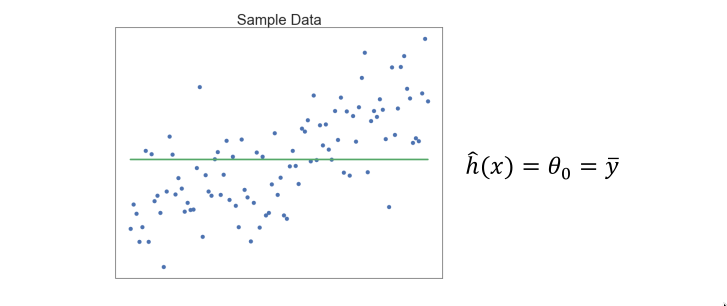
\includegraphics[width=0.8\textwidth]{assets/mean_predictor_df.png}
  \caption{Mean Predictor}
  \label{fig:mean_predictor_df}
\end{figure}
  # TODO OLS and later
\end{note}

\subsection{Identity Predictor}
\begin{note}
  Another example is an \textbf{identity} estimator like $\hat{y}^i = f(x^i) = y^i$ has $N$ degrees of freedom:
   \[
     df(\hat{h}) = \frac{1}{\sigma^2} \sum_{i=1}^N Cov(\hat{y^i}, y^i) = \frac{1}{\sigma^2} \sum_{i=1}^N Cov(y^i, y^i) = \frac{1}{\sigma^2}\sum_{i=1}^N \sigma^2 = N
  .\] 
\end{note}

\subsection{OLS Degrees of Freedom}
\begin{note}{OLS Example} \\
  Let $\hat{y} = X \hat{\vec{\theta}} = X(X^TX)^{-1} X^T \vec{y}$ :
  \begin{align*}
    df(\hat{h}) &= \frac{1}{\sigma^2} Tr(Cov(\hat{\vec{y}}, \vec{y})) \\
                &=
  .\end{align*}
  TODO finish notes here
\end{note}

\subsection{Linear Smoother DoF}
Note that $\w\left(  \right)$ is a special function, essentialy acting as a weighted average!

\begin{definition}
  A model call linear smoother has forms:
  \begin{align}
    & \hat{f}\left( \vec{x} \right) = \sum_{j=1}^N w(\vec{x}, \vec{x}^j) \cdot y^j \\
    & \hat{f}\left( \vec{x}^i \right) = \sum_{j=1}^N w(\vec{x}^i, \vec{x}^j) \cdot y^j \\
    & \hat{f}\left( \vec{x} \right) = \hat{\vec{y}} = W \vec{y} 
  \end{align}
  where (1)-(3) are equivalent forms!
\end{definition}

TODO Derivation of the degrees of freedom
\begin{proof}
  TODO
\end{proof}

\subsection{K-Nearest Neighbors DoF}
\begin{remark}
  Actually a K-Nearest Neighbors is a \textbf{special case} of the linear smoothers.
\end{remark}

Recall,
\[
  \hat{f}(\vec{x}) = \frac{1}{k} \sum_{\vec{x}^j \in N_0} y^j 
.\] 
In fact, this is just equal to $\sum_{j=1}^N w\left( \vec{x}, \vec{x}^j \right) \cdot  y^{j}$  where
\[
  w\left( \vec{x}, \vec{x}^j \right) = \begin{cases}
    \frac{1}{k} \text{ if $\vec{x}^j \in N_0$} \\
      0 \text{ otherwise}
  \end{cases} 
.\] 

\begin{remark}
  If $k=1$, then it is the \textbf{identity predictor}. If $k=N$ then it is the \textbf{mean} predictor!
\end{remark}

\begin{proof}
  TODO Expand and rigorize proof
  \begin{align*}
    df(\hat{\vec{y}} = Tr(W) = \frac{N}{K}
  .\end{align*}
\end{proof}

\section{Estimating Degrees of Freedom}
While we do have a theoretical formula (in the definition) for the degrees of freedom, in many 
models, there is no analytic calculation.

We can estimate the degrees of freedom through simulation! I.e. using random resampling 
(taking one datapoint in $D_1, D_2, \ldots$) in something called the \textbf{bootstrap} method.
 \[
   Cov(x,z)_{\text{sample}} = \frac{\sum_{i=1}^B (x_i - \overline{x})\left( z_i - \overline{z} \right) }{B-1}
.\] 

\begin{note}{Procedure}\\
  For $B=1$ to $B=N$:
  \begin{enumerate}
    \item Draw samples $\left( \vec{x}_b^i, y_b^i \right) $ for $i=1,\ldots,N$
    \item Compute $\hat{\vec{y}}_b = \begin{pmatrix} h(\vec{x}^1_b)\\ \vdots\\ h(\vec{x}^N_b) \end{pmatrix}$ 
      and $\vec{y}_b\begin{pmatrix} y_b^1\\ \vdots\\ y_b^N \end{pmatrix}$\
    \item Calculate using the following:
  \end{enumerate}

  \begin{align*}
    df(\hat{h}) &= \frac{1}{\sigma^2} \sum_{i=1}^N Cov(\hat{y}^i, y^i) \\
                &= \frac{1}{\sigma^2} \sum_{i=1}^N Cov_{\text{sample}} \left(\hat{y}^i, y^i \right) \\
                &= \frac{1}{\sigma^2} \sum_{i=1}^N \frac{1}{B-1} \sum_{b=1}^B \left( \hat{y}_b^i - \overline{y}_b^i  \right) 
                \left( y_b^i - \overline{y}_b^i \right) 
  .\end{align*}
  Note: May also have to estimate variance using the sample in practice!
\end{note}

\section{Training and Test Error}
Let $D = \{\vec{x}^i, y^i\}, i = 1,\ldots,N$ the training data.
\begin{definition}{Sample training Error} \\
  Defined as the average error of our $\hat{f}(x)$ on training points $D$:
  \[
    err_D = \frac{1}{N} \sum_{i=1}^N L(y^i, \hat{f}(\vec{x}^i))
  .\] 
\end{definition}

\begin{definition}{Expected Test Error} \\
  Final Goal in theory! Defined as the expected error on future data (impossible) points $(\vec{X}, Y)$ based on
  current fixed training set $D$:
   \[
     Err_D = E(L(Y, \hat{f}(\vec{X})))
  .\] 
  Averaging over all possible $D$ is just called \textbf{Err} $E_D(Err_D)$
\end{definition}
\begin{definition}{In Sample Prediction Error} \\
  A mix of Test Error and the theoretical Expected Test Error. Still not computable, but closer
  \[
    Err_in =\frac{1}{N} \sum_{i=1}^N E_{Y_{new}} (L(Y_{new}^i, \hat{f}(\vec{x}^i)))
  .\] 
  Expected error based on same function $\hat{f}\left( \vec{x}^i \right) $ from $D$ with same $\vec{x}^i$
  but newly generated  $y_{new}^i$ from the underlying distribution (this is the unrealistic assunption part).
\end{definition}

\begin{definition}{Optimism} \\
  The difference between test and training errors is known as \textbf{optimism} of estimator $\hat{h}$.
  \[
  optimism = Err_{in} - err_D = \frac{1}{N} \sum_{i=1}^N E_{Y_{new}} (L(Y_{new}^i, \hat{f}(\vec{x}^i))) - \frac{1}{N} \sum_{i=1}^N L(y^i, \hat{f}(\vec{x}^i))
  .\]  
\end{definition}

\begin{theorem}{Optimism and Degrees of Freedom}\\
  We are averaging over all $y_i$ in $D$:
  \[
  E_y(Optimism) = \frac{2}{N} \sum_{i=1}^N Cov(\hat{y}^i, y^i) = \frac{2 \sigma^2}{N} df(\hat{f})
  .\]
Derivation:
\begin{align*}
  E_y(Err_{in} - err_D) &= E_y(Err_{in} - err_D) \\
                        &= E_y[\frac{1}{N} \sum_{i=1}^N E_{Y_{new}} (L(Y_{new}^i, \hat{f}(\vec{x}^i)))] - E_y[\frac{1}{N} \sum_{i=1}^N L(y^i, \hat{f}(\vec{x}^i))] \\
                        &= \frac{2 \sigma^2}{N} df(\hat{f})
.\end{align*}
\end{theorem}

\subsection{Mean Square Error Example}
We can find $Err_{in}=err_D + \frac{2 \sigma^2}{N} df(\hat{f}) \approx T$:
\[
T=\frac{1}{N} \sum_{i=1}^N L(y^i, \hat{f}(\vec{x}^i)) +  \frac{2 \sigma^2}{N} df(\hat{f}) 
.\]
By optimism, where $L\left(y^i, \hat{y}^i \right) = (y^i - \hat{y}^i)^2$
\begin{align*}
  E[Err_{in}] & \approx E[T] \\
              &= E[\frac{1}{N} \sum_{i=1}^N L(y^i, \hat{f}(\vec{x}^i)) +  \frac{2 \sigma^2}{N} df(\hat{f})] \\
              &=  E[\frac{1}{N} \sum_{i=1}^N L(y^i, \hat{f}(\vec{x}^i))] \\
              &= \text{ TBH don't really understand the steps}
.\end{align*}
And it is an unbiased estimator!


Thus, if we knew the estimators DoF, then we can use T to approximate test error!

\begin{definition}
  The \textbf{Cp information criterion} for model selection in linear regression is then just defined as ($df(f_k) = k$ since in lin reg, the dof = num params):
  \[
    \hat{k} = \arg\min_{k} \frac{1}{N} \sum_{i=1}^N (y^i - \hat{y}^i)^2 + \frac{2 \sigma^2}{N} k
  .\] 
\end{definition}

\section{AIC Criterion for Log}
A test error estimate. Generally, for log-likelihood models.

\section{VC Dimension}
Before: We want estimate for $Err_{in}$ in terms of training set and correction term. 

\begin{remark}
  $VC$ gives an upper bound of \textbf{full Ex[ected Test Error} i.e.
\[
Err = E_{Y,\vec{X}} (L(Y, \hat{f}(\vec{X})))
.\] 
\end{remark}

\begin{definition}
 \textbf{indicator} functions are defined as:
  \[
    f(\vec{x}) = \begin{cases}
      1 \text{  if $\vec{x} \in A$} \\ 
      0 \text{  otherwise}
    \end{cases}
  .\] 
   
\begin{figure}[H]
  \centering
  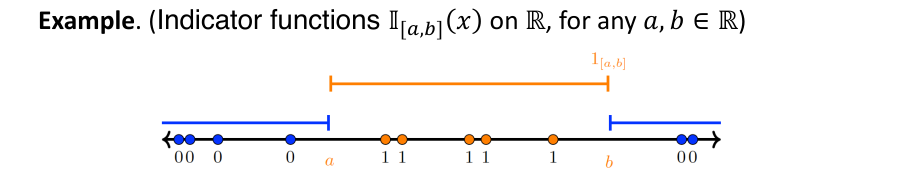
\includegraphics[width=0.8\textwidth]{assets/indicator_function_example.png}
  \caption{Ex: Indicator Function}
  \label{fig:indicator_function_example}
\end{figure}
\end{definition}

\begin{definition}
  A family $F$ of indicator functions  $f\left( \vec{x} \right) = I_A (\vec{x}) $ on $\R^{d}$ shatters
  a fixed finite collection of points $C$ if the  following holds:

  For every subset $C_1 \subseteq C$,  $\exists$ a function  $I_{A} (\vec{x})$ in family with $1$ on 
   $C_1$ and  $0$ on  $C \setminus C_1$.

  In terms of estimating model complexity, what this equates to is the indicator function being our model
  (ex: $y = \theta_1 x_1 + \theta_2 x_2 + \theta_0$) and the family of indicator functions being
  all possible values for parameters  $\theta$. Then the collection of points we attempt to shatter
  are analogous training set datapoints where $1$ represents the points we want classify correctly using model and $0$
  representing all the points outside. So can the model correctly classify all possible labellings of 
  arbitray number of points and the maximum number possible is $VC$ dimension
\end{definition}

TODO can't screenshot tool working 
\begin{figure}[h]
  \centering
  \includegraphics[width=0.8\textwidth]{assets/VC_dim_shattering_example.png}
  \caption{VC Dimension of 2 (can't shatter the right example! Since interval must be continuous)}
  \label{fig:vc_dim_shattering_example}
\end{figure}

\begin{note}
  \begin{itemize}
    \item What about when indicator functions of circle with radius $r \in \R^+$ centered at $\left( 0,0 \right) $? 
      VC Dim = 1, can't classify the point further away as being in the circle with the point closer as not
    \item What about if the circles could have the center vary $(a,b) \forall a,b \in \R$?
      VC Dim = 3, can't classify 4.
    \item How about 3-dimensional balls with radius $r \in \R^+$ centered at $\vec{0}$?
  \end{itemize}
\end{note}

\begin{definition}
  The family $F$ of indicator functinos has \textbf{VC Dimensions} $n$ if $n$ is largest number of points $F$ 
  can always shatter. It can be thought of a way of measuring complexity of a class of functions by
  measuring how wiggly its members can be.
\end{definition}

\begin{figure}[h]
  \centering
  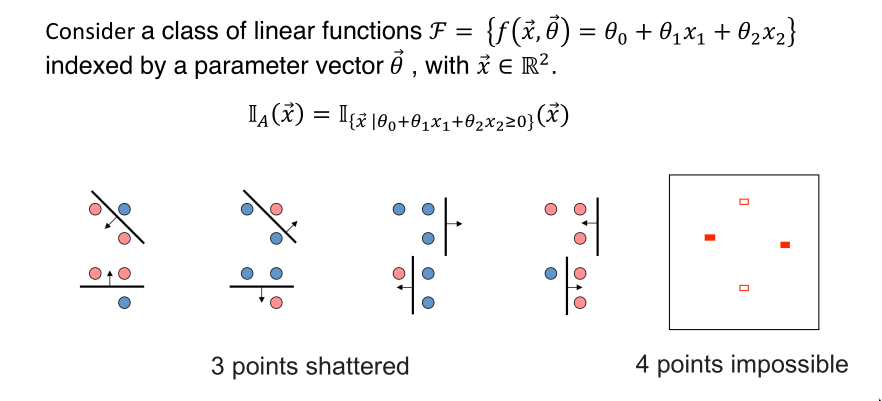
\includegraphics[width=0.8\textwidth]{assets/2024-09-18-12-22-21.png}
  \caption{VC dimension Example for Linear functions}
  \label{fig:2024-09-18-12-22-21}
\end{figure}
\begin{note}
  Thus, the VC dimension of a linear model is as expected: $VC = d + 1$ where $\theta_1, \ldots, \theta_d$
\end{note}

However, in general, the number of paramters is not always approximate of the VC dimensions! For example,
consider the classifer:
\[
  f(x,a) = \left\lceil \sin(ax) \right\rceil \text{ i.e. the ceiling} 
.\] 
which has only 1 parameter, but infinite VC dimesion

\subsection{VC Dimesion Bound}
\begin{definition}{Error Bound}
  \[
    err_{\text{test}} \leq err + \frac{\epsilon}{2} \left( 1+ \sqrt{1+ 4 \cdot \frac{err}{\epsilon}}  \right) 
  .\] 
  Thus, VC Dimensions give an upper bound for the test error based on training error
\end{definition}
\begin{note} This is only for binary classification
  
\end{note}


\end{document}
